\section{Results and Discussion}
All three methods were applied to five meteorological variables across
all facilities. The methods identified different sets of outlier events,
with some events identified by more than one methods
(Figures~\ref{fig:pc},\ref{fig:ssa},\ref{fig:kmeans}).

Among three methods Pearson correlation was least effective with
frequent false negatives. Pearson correlation is also an aggressive method that
it may include many false positives. Those are all due to the fact 
that pairwise Pearson correlation method was applied at seasonal scale.
Pearson correlation coefficient is a pairwise comparison method, however, 
if the two variables deviate in the same direction, their correlation 
may not change significantly and thus may go undetected. Due to seasonal
nature of the analysis, it was not able to identify outliers that
persisted at hours to days only. Univariate SSA method was very effective 
at identifying outliers with extreme high and low values in the time series 
but required the input data to be consistent with no missing values.
$k$-means could be used to detect extreme storms and weather events but it was hard
to tell which variable mainly caused the abnormality. However, these drawbacks 
could be easily overcome by combining methods together to detect 
outliers from three different angles.

\begin{table}[ht]
\caption{Comparison of SSA and K-means Outlier Set Size}
\label{tab:comp}
\centering
\begin{tabular}{|l|c|}
\cline{2-2}
\multicolumn{1}{l|}{} & Outlier Set Size\\
\hline
SSA & 922\\
K-means & 508\\
Intersection & 378\\
Symmetric Difference & 674\\
\hline
\end{tabular}
\end{table}

\begin{table*}[ht]
\caption{Precision and Recall of SSA and K-means}
\label{tab:pr}
\centering
\begin{tabular}{|l|c|c|c|c|c|}
\hline
Method & Variable & Database Entries & Affected Days & Precision & Recall\\
\hline
SSA & temp\_mean & 41 & 8217 & 16.00\% & 1.20\%\\
SSA & vapor\_pressure\_mean & 42 & 8194 & 20.70\% & 1.40\%\\
SSA & atmos\_pressure & 12 & 76 & 0.00\% & 0.00\%\\
SSA & rh\_mean & 32 & 8108 & 14.80\% & 0.50\%\\
SSA & wspd\_arith\_mean & 52 & 265 & 0.60\% & 1.50\%\\
Kmeans & 5 together & 181 & 8540 & 13.00\% & 1.90\%\\
Combined & 5 together & 181 & 8540 & 11.10\% & 4.10\%\\
\hline
\end{tabular}
\end{table*}

In our experiment, SSA method identified largest number of outlier events (922)
(Table~\ref{tab:comp}) across the entire dataset, while $k$-means
identified 508 events. While 378 events were identified as outlier by
both the methods (intersection), 674 events were only identified by one
of the methods (Table~\ref{tab:comp}).
Figure~\ref{fig:combined} shows all the outliers detected by Pearson correlation, SSA and
$k$-means methods at facility E33 for air temperature. 
%We can see from Figure~\ref{fig:combined}
%that spring 2015 was treated as outlier season by Pearson correlation
%due to large temperature fluctuation due to spring frost event. 
When using Pearson Correlation, we used 
the interquartile range (IQR) method to extract outlier seasons that 
is those values beyond Tukey's fences as the three sigmas rule is too 
aggressive for Pearson correlation \cite{tukey1977exploratory}. 
However, since the Pearson Correlation was applied at seasonal scale it
identified only a few outlier seasons in the data. For example, at
facility E33 Pearson Correlation analysis of temperature time series
identified spring 2015 that experienced a severe frost event as outlier
season (Figure~\ref{fig:combined}).
When combined together SSA and $k$-means methods had \textit{Precision} of 
11.10\% which shows that many of the outliers
detected are not within ARM DQR database, which is a known limitation of
the current records that this current study is trying to address.
Detected outliers also had low \textit{Recall} which in addition to small
number of true positives can be due to fact that DQR database often
records a wide affected date range for an identified outlier instead of a
precise date thus leading to large false negatives, all of which leads
to low \textit{Recall} values.

Overall, when combined together within a framework, set of methods applied allows
to capture outlier events caused by a wide range of conditions. 

\begin{figure*}[ht]
    \centering
    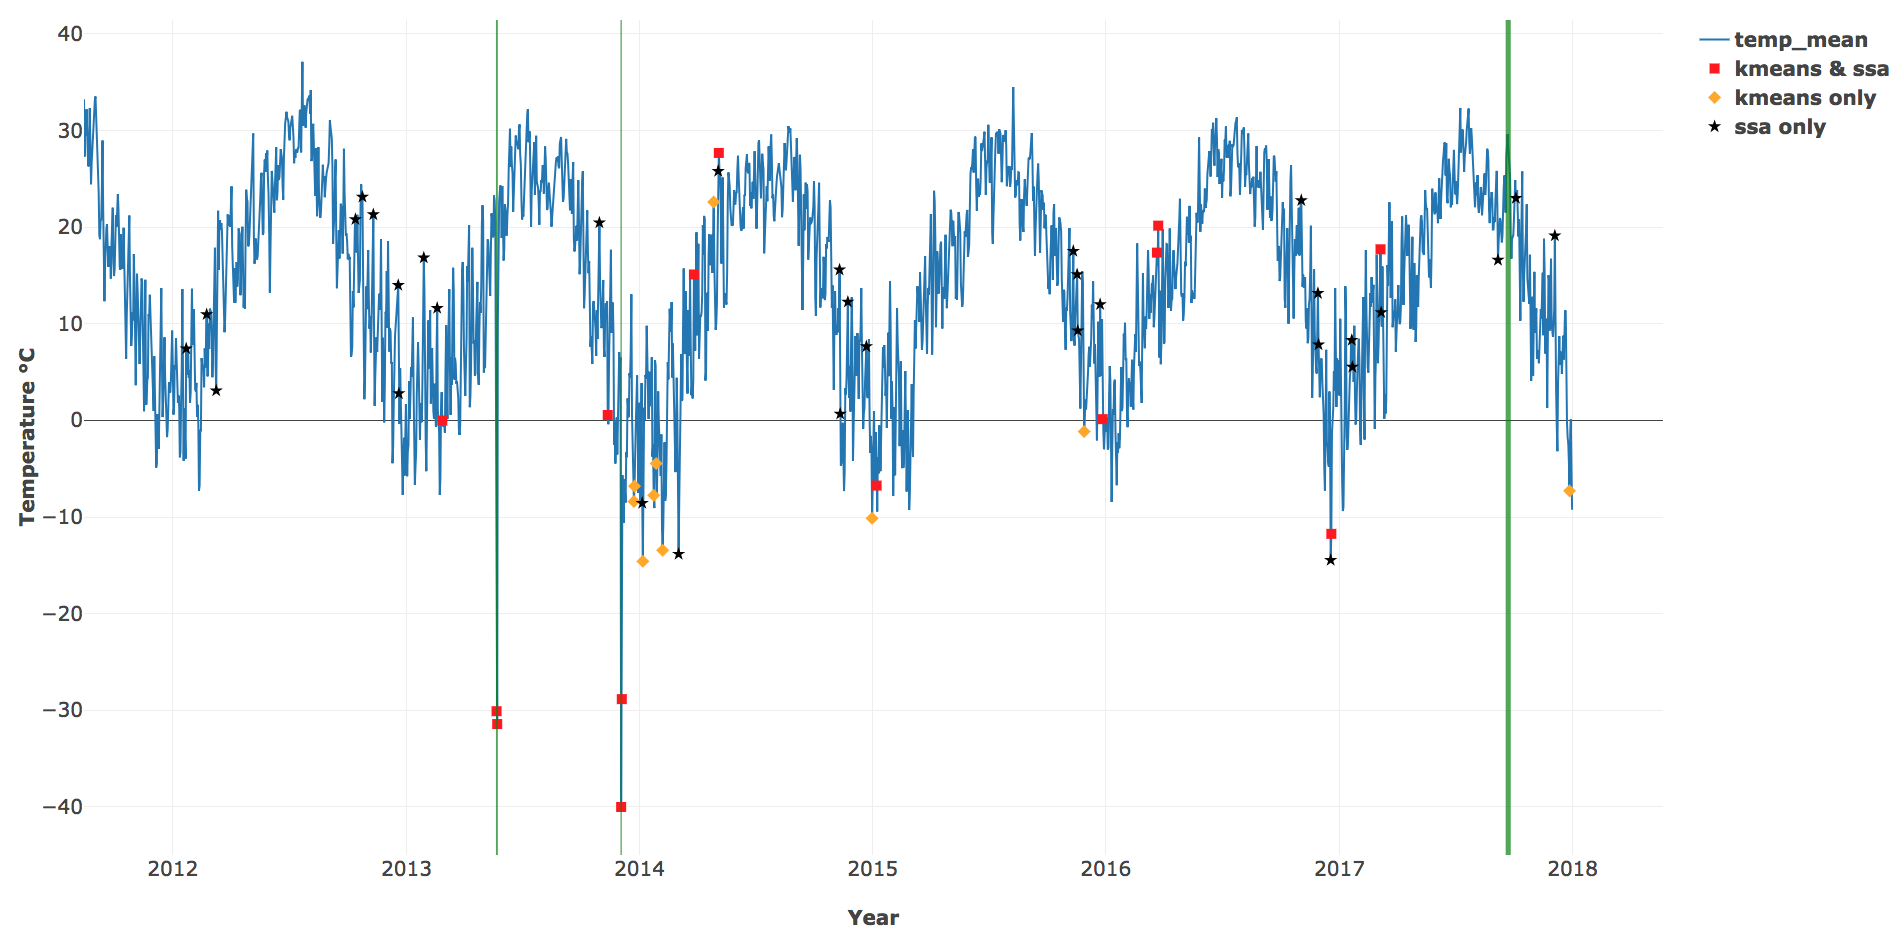
\includegraphics[width=\textwidth]{figures/combined.png}
    \caption{Outliers detected at facility E33 for air temperature
		by Pearson correlation, SSA and $k$-means algorithms. The yellow shaded areas are
		outliers detected by Pearson correlation. Outliers detected by both SSA and $k$-means
		algorithms are shown by red squares, while those identified by
		SSA and $k$-means only are indicated by black stars and orange
		diamonds respectively. DQR records are denoted by the vertical green shaded areas.}
    \label{fig:combined}
\end{figure*}
